%versi 2 (8-10-2016)
\chapter{Landasan Teori}
\label{chap:teori}

Pengelompokan dokumen berkaitan erat dengan dua bidang ilmu dalam informatika. Pe-ngelompokan dalam informatika merupakan bagian dari bidang pembelajaran mesin. Terdapat dua jenis pengelompokan dalam pembelajaran mesin yaitu \textit{clustering} dan \textit{classification}. \textit{Clustering} merupakan salah satu jenis pembelajaran tak terarah (\textit{unsupervised learning}) karena setiap elemen dikelompokkan berdasarkan karakteristik dari elemen tersebut. Sedangkan \textit{classification} merupakan jenis pembelajaran terarah (\textit{supervised learning}) karena setiap elemen dikelompokkan berdasarkan label yang telah ditentukan sebelumnya. Pada penelitian ini, jenis pengelompokan yang akan digunakan adalah \textit{clustering}.

\section{Pengelompokan}
\subsection{Definisi Pengelompokan}
Pengelompokan (\textit{clustering}) merupakan sebuah metode untuk menggabungkan himpunan objek ke dalam kelompok-kelompok sedemikan rupa sehingga objek dalam kelompok (\textit{cluster}) lebih mirip (karena suatu hal) satu sama lain daripada objek di kelompok lain \cite{gan2007data}. Pengelompokan seringkali tertukar dengan istilah klasifikasi yang hanya bertugas untuk memisahkan objek ke dalam kelas-kelas yang telah ditentukan sebelumnya. Masukan dari proses pengelompokan adalah kumpulan objek dan banyaknya kelompok (\textit{cluster}) yang akan dibentuk. Keluaran yang dihasilkan dari proses pengelompokan adalah kelompok objek yang telah dibentuk beserta anggotanya. Setiap objek dikelompokkan berdasarkan kesamaan tertentu. Sebagai ilustrasi dari pengelompokan (Gambar \ref{fig:cluster}), terdapat tiga \textit{cluster} yang ditandai dengan warna merah, biru, dan hijau. Objek-objek yang berwarna sama dianggap mirip sehingga dimasukkan ke dalam kelompok yang sama. Begitu juga dengan objek yang berbeda warna dianggap tidak mirip sehingga perlu dipisahkan.

\begin{figure}[h]
	\begin{center}
		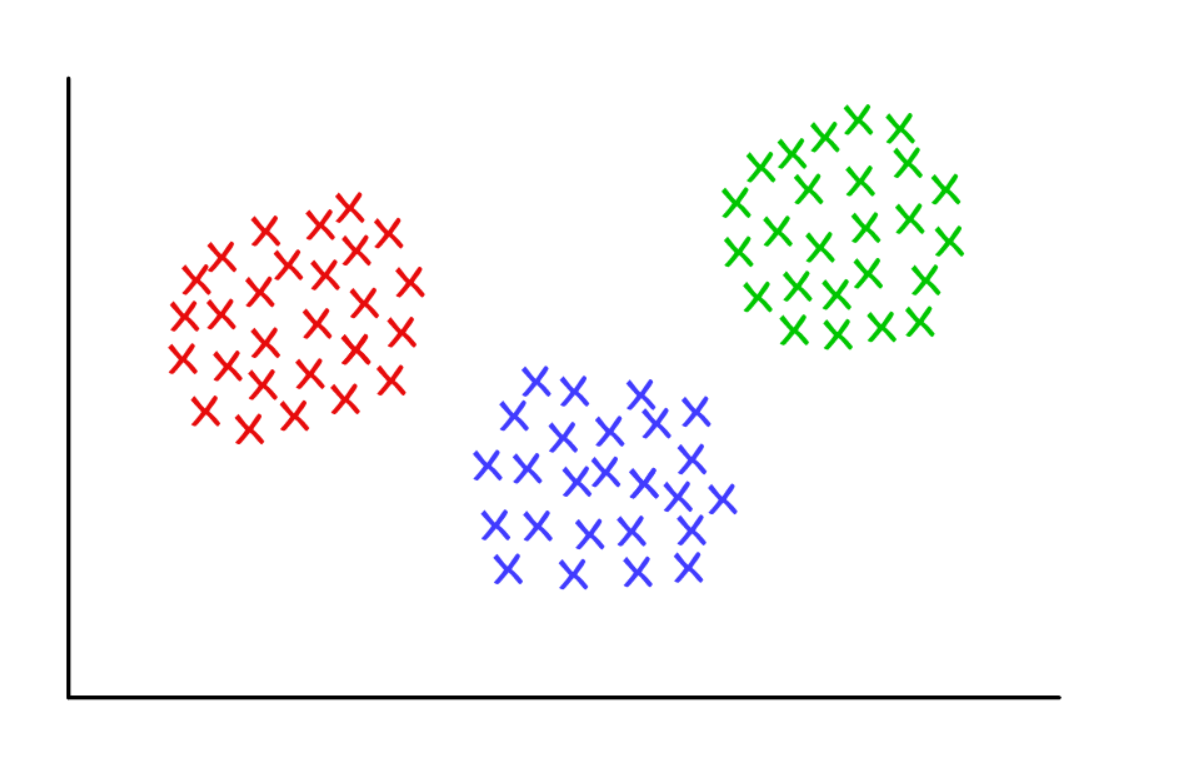
\includegraphics[width=0.4 \textwidth]{cluster}
		\caption{Contoh \textit{cluster} hasil pengelompokan}
		\label{fig:cluster}
	\end{center}
\end{figure}

\subsection{Aplikasi Pengelompokan}
Pengelompokan memegang peran penting dalam beberapa bidang seperti \textit{recommender system} dan penambangan data. Berikut adalah penjelasan singkat aplikasi pengelompokan dalam setiap bidang yang telah disebutkan.

\subsubsection{\textit{Recommender System}}
\textit{Recommender system} adalah suatu sistem yang berfungsi untuk memprediksikan keinginan pengguna berdasarkan masukkan yang diberikan oleh pengguna \cite{zhai2016text}. Ada dua jenis sistem rekomendasi yaitu \textit{Content-based Recommendation} dan \textit{Collaborative Filtering}.

\begin{itemize}
	\item \textit{Content-based Recommendation}: mempelajari apa yang pengguna sukai lalu mencari objek lain yang mungkin juga disuka oleh pengguna tersebut berdasarkan apa yang disukainya. Pencarian ini dilakukan dengan mengusulkan objek-objek yang berada dalam kelompok (\textit{cluster}) yang sama dengan objek yang disukai oleh pengguna. Hal ini dilakukan dengan asumsi pengguna akan menyukai barang yang mirip dengan barang yang disukainya.
	\item \textit{Collaborative Filtering}: memberikan usulan berdasarkan apa yang disukai pengguna yang serupa dengan seseorang dengan mengasumsikan jika pengguna serupa menyukai suatu objek, maka orang tersebut akan menyukai objek yang sama. Pengguna serupa didapatkan dengan mencari orang-orang yang berada dalam satu \textit{cluster} dengan memperhitungkan atribut dari pengguna (usia, jenis kelamin, tempat domisili, hobi, dll).
\end{itemize}


\subsubsection{\textit{Search Result Clustering}}
Salah satu kegunaan pengelompokan dalam bidang penambangan data adalah untuk mengelompokan hasil pencarian (\textit{search result clustering})\cite{mecca2007new}. Setiap kata kunci dalam sebuah pencarian mungkin dapat masuk ke dalam berbagai kategori. Misalkan kata kunci "\textit{apple}" dapat berarti buah apel atau perusahaan teknologi \textit{apple}. Dengan menggunakan pengelompokan hasil pencarian, maka hasil dari pencarian akan dimasukkan ke dalam kelompok-kelompok topik dan pengguna dapat memilih topik mana yang dimaksud untuk dapat mengeluarkan hasil yang lebih spesifik. Mesin pencari yang mengelompokan hasil pencariannya dinamakan dengan \textit{clustering search engine}. Salah satu contoh \textit{clustering search engine adalah} Yippy\footnote{\href{https://yippy.com/}{https://yippy.com/}}. 

\begin{figure}[h]
	\centering
	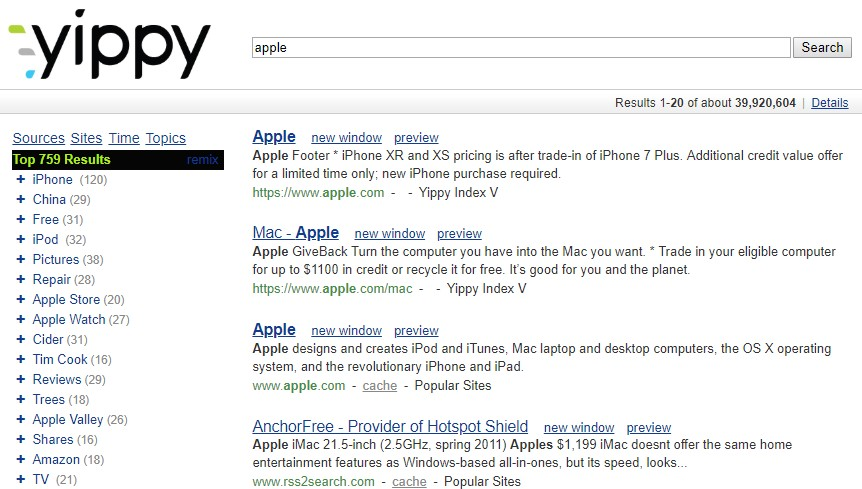
\includegraphics[width=.69\linewidth]{clustered-search}
	\caption{Hasil pencarian (\textit{clustered search result}) di Yippy}
	\label{fig:yippy}
\end{figure}

Hasil pencarian di Yippy dengan kata kunci "\textit{apple}" ditunjukkan dalam Gambar \ref{fig:yippy}. Bagian sebelah kiri pada Gambar \ref{fig:yippy} merupakan kelompok-kelompok kategori dari kata kunci yang dimasukkan sehingga pengguna dapat memilih kategori yang sesuai dengan yang mereka maksud. "\textit{iPhone}", "\textit{China}", "\textit{Free}", dan seterusnya merupakan kelompok yang dihasilkan apabila pengguna memasukkan kata kunci "\textit{apple}".

\subsection{\textit{Local Optimum}}
\textit{Local optimum} adalah suatu solusi yang optimal (baik maksimal maupun minimal) diantara kandidat solusi yang berdekatan dalam masalah optimasi. Dikatakan lokal karena solusi ini hanya optimal apabila dibandingkan dengan kandidat solusi yang berdekatan, tidak optimal secara keseluruhan (\textit{global optimum}). Contoh dari \textit{local} dan \textit{global} optimum ditunjukkan pada Gambar \ref{fig:optima}. \textit{Local minimum} memiliki nilai yang paling kecil apabila dibandingkan dengan nilai-nilai lain yang berdekatan dengannya, begitu pula dengan \textit{local maximum}. Sedangkan \textit{global minimum} dan \textit{global maximum} memiliki nilai yang paling minimum dan maksimum dalam keseluruhan himpunan kandidat solusi.

\begin{figure}[h]
	\begin{center}
		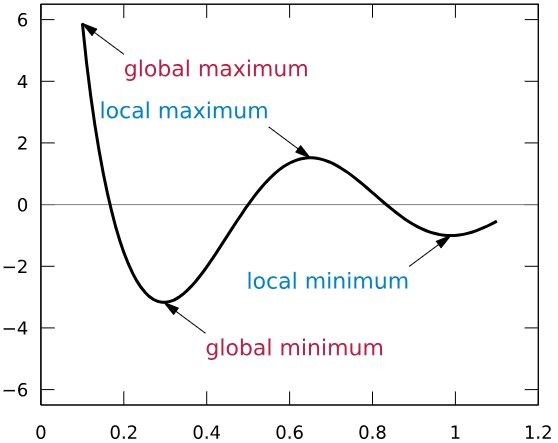
\includegraphics[width=0.4 \textwidth]{local-optima}
		\caption{\textit{Local Optimum} dan \textit{Global Optimum}}
		\label{fig:optima}
	\end{center}
\end{figure}

Suatu program optimasi dapat terjebak di \textit{local optimum}. Sebagai contoh pada Gambar \ref{fig:optima}, apabila suatu program mencari solusi yang merupakan nilai maksimum maka program dapat terjebak pada nilai $2$ yang merupakan \textit{local maximum} karena seharusnya keluaran dari program tersebut adalah $6$ yang merupakan \textit{global maximum}. Sedangkan apabila suatu program mencari solusi berupa nilai minimum maka program dapat terjebak pada nilai $-1$ yang merupakan \textit{local minimum} karena seharusnya keluaran dari program tersebut adalah $-3$ yang merupakan \textit{global minimum}.

\section{\textit{K-Means}}
\textit{K-means} merupakan salah satu algoritma pengelompokan yang umum digunakan saat ini. Algoritma ini membagi objek ke dalam $K$ \textit{cluster}. Setiap \textit{cluster} direpresentasikan dengan titik tengahnya (\textit{centroid}). Titik tengah akan dihitung sebagai rata-rata dari semua titik objek dari \textit{cluster} tersebut dalam setiap iterasinya. Persamaaan \ref{eq:kmeans} merupakan persamaan untuk menghitung \textit{centroid}
\begin{equation}
	\label{eq:kmeans}
	\mu_i=\frac{1}{N_i}\sum_{q=1}^{N_i}x_q
\end{equation}
dengan $\mu_i$ merupakan \textit{centroid} ke-$i$, $N_i$ merupakan jumlah titik objek pada \textit{cluster} ke-$i$, dan $x_q$ merupakan titik ke-$q$ pada \textit{cluster} ke-$i$.

\begin{algorithm} % enter the algorithm environment
\caption{\textit{K-means}} % give the algorithm a caption
\label{alg:kmeans} % and a label for \ref{} commands later in the document
\begin{flushleft}
	\textbf{Input:} $S$ (himpunan titik objek), $K$ (Jumlah \textit{cluster})\\
	\textbf{Output:} himpunan \textit{cluster}
\end{flushleft}
\begin{algorithmic}[1] % enter the algorithmic environment
	\STATE Pilih $K$ titik objek sebagai himpunan awal \textit{centroid}. \label{alg:kmeans:ln-1}
	\REPEAT \label{alg:kmeans:ln-2}
		\STATE Bentuk $K$ \textit{cluster} dengan menempatkan setiap titik objek ke \textit{cluster} dengan \textit{centroid} terdekat. \label{alg:kmeans:ln-3}
		\STATE Hitung ulang \textit{centroid} untuk setiap \textit{cluster}. \label{alg:kmeans:ln-4}
	\UNTIL{\textit{Centroid} tidak berubah.} \label{alg:kmeans:ln-5}
\end{algorithmic}
\end{algorithm}

Penjelasan dari Algoritma \ref{alg:kmeans} adalah sebagai berikut:
\begin{itemize}
	\item Pada baris \ref{alg:kmeans:ln-4}, \textit{centroid} baru akan ditentukan dengan menggunakan Persamaan \ref{eq:kmeans}.
	\item Pada baris \ref{alg:kmeans:ln-5}, pengulangan akan berhenti saat \textit{centroid} mengalami pergeseran yang tidak terlalu signifikan (lebih kecil dari suatu nilai $\epsilon$ yang merupakan masukan dari pengguna).
\end{itemize}

\section{Algoritma Genetika}
\label{sec:GA}
Algoritma genetika atau biasa disebut \textit{Genetic Algorithm}(GA) adalah suatu algoritma pencarian yang terinspirasi dari proses seleksi alam yang terjadi secara alami dalam proses evolusi. Di alam, individu dalam suatu populasi berkompetisi satu sama lain untuk memperebutkan tempat tinggal, makanan, dll \cite{sivanandam2007introduction}. Bahkan setiap individu dalam spesies yang sama pun harus bersaing menarik lawan jenis untuk berkembang biak. Individu yang kurang baik akan memiliki peluang bertahan hidup lebih kecil, dan individu yang bisa beradaptasi dengan baik atau "\textit{fit}" akan menghasilkan keturunan dengan jumlah yg relatif banyak. 

GA merupakan metode penyelesaian masalah yang menggunakan genetika sebagai pemodelannya. Suatu calon solusi dalam GA dimodelkan sebagai suatu individu. Kumpulan individu-individu ini disebut dengan populasi. Setiap individu dalam populasi direpresentasikan dengan kromosom. Kromosom merupakan kumpulan parameter yang membentuk suatu solusi. Parameter-parameter yang menyusun kromosom disebut dengan gen. Setiap kromosom memiliki suatu nilai yang terkait dengan \textit{fitness} dari solusi yang direpresentasikannya. Nilai itu biasanya disebut dengan nilai \textit{fitness}.

%Individu yang lebih "kuat" akan memiliki peluang terpilih lebih besar dalam proses seleksi. Individu yang terpilih pada proses seleksi akan disilangkan untuk menghasilkan keturunan. Keturunan yang dihasilkan pada proses persilangan dapat memiliki peluang untuk mengalami mutasi. Setelah itu, akan dilakukan proses evaluasi terhadap nilai \textit{fitness} dari setiap kromosom untuk menentukan apakah solusi yang baik sudah ditemukan atau belum. Proses ini akan diulang terus-menerus untuk setiap generasi sampai ditemukan solusi yang sudah optimal. Secara umum, \textit{flowchart} dari GA ditunjukkan pada Gambar \ref{fig:GA-flowchart}.

\begin{figure}[H]
	\centering
	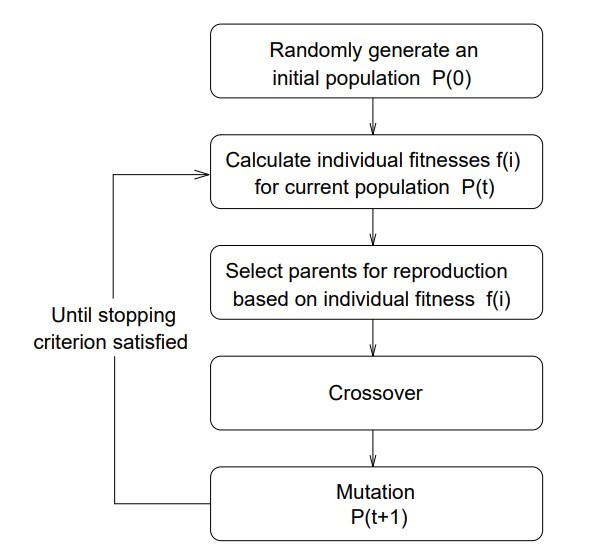
\includegraphics[width=0.45 \textwidth]{GA-flowchart2}
	\caption{Alur algoritma genetika dasar}
	\label{fig:GA-flowchart}
\end{figure}

Secara umum, proses pada GA ditunjukkan dalam Gambar \ref{fig:GA-flowchart}. Penjelasan dari proses-proses pada GA yang disebutkan dalam Gambar \ref{fig:GA-flowchart} adalah sebagai berikut:

\begin{enumerate}
	\item \textbf{Inisialisasi Populasi} \\
	Inisialisasi populasi merupakan tahap paling awal dari GA. Pada proses ini, akan dibentuk populasi $P(0)$ secara acak. 
	\item \textbf{Perhitungan \textit{Fitness}} \\
	Menghitung nilai \textit{fitness} $\textrm{f}(i)$ dari setiap individu dalam populasi saat ini $P(t)$. Nilai \textit{fitness} ini akan digunakan dalam operasi genetik selanjutnya.
	\item \textbf{Seleksi} \\
	Proses seleksi akan terjadi berdasarkan nilai \textit{fitness} $\textrm{f}(i)$ setiap individu. Individu yang lebih \textit{fit} akan memiliki peluang terpilih lebih besar dalam proses seleksi.
	\item \textbf{Persilangan} \\
	Individu yang terpilih pada proses seleksi akan disilangkan untuk menghasilkan keturunan. Proses persilangan ini terjadi antara dua induk hasil seleksi.
	\item \textbf{Mutasi} \\
	Keturunan yang dihasilkan pada proses persilangan dapat memiliki peluang untuk mengalami mutasi. Mutasi dapat terjadi dengan suatu peluang terjadinya mutasi.
\end{enumerate}

Proses 2 sampai 5 akan diulang terus-menerus sampai ditemukan suatu solusi yang optimal. Berikut merupakan penjelasan lebih lanjut mengenai istilah yang ada pada GA.

\subsection{\textit{Fitness}}
\label{sub:fitness}
\textit{Fitness} dari suatu individu dalam algoritma genetika adalah suatu nilai fungsi objektif untuk fenotipenya \cite{sivanandam2007introduction}. \textit{Fitness} harus bisa memperkirakan seberapa dekat sebuah calon solusi dengan solusi yang optimal. Suatu solusi yang optimal akan memaksimalkan fungsi \textit{fitness}. Perhitungan \textit{fitness} sangatlah tergantung dengan masalah yang ingin diselesaikan. Fungsi \textit{fitness} yang baik harus bisa menentukan solusi mana yang paling baik diantara banyak calon solusi.

\subsection{Seleksi}
\label{sub:selection}
Seleksi adalah proses pemilihan dua induk dari populasi untuk disilangkan \cite{sivanandam2007introduction}. Tujuan dari proses seleksi adalah untuk menonjolkan individu yang memiliki nilai \textit{fitness} tinggi dalam populasi dengan harapan keturunannya akan memiliki \textit{fitness} yang lebih tinggi. Seleksi adalah suatu metode yang memilih kromosom secara acak dari populasi berdasarkan fungsi \textit{fitness}. Semakin tinggi fungsi \textit{fitness} maka semakin tinggi peluang suatu individu akan terpilih. 

Salah satu teknik yang populer digunakan dalam seleksi adalah \textit{roulette-wheel selection} atau \textit{fitness proportional selection}. \textit{Roulette-wheel selection} memilih suatu individu dari populasi dengan probabilitas yang sebanding dengan nilai \textit{fitness} relatifnya. Berdasarkan ilustrasi yang terdapat dalam Gambar \ref{fig:pieChart}, setiap individu memiliki sebuah bagian pada diagram sesuai dengan nilai \textit{fitness} relatif. Semakin tinggi nilai \textit{fitness}, maka semakin besar bagian yang dialokasikan dan semakin besar kemungkinan individu tersebut akan terpilih dalam proses seleksi.

\begin{figure}[H]
	\begin{center}
		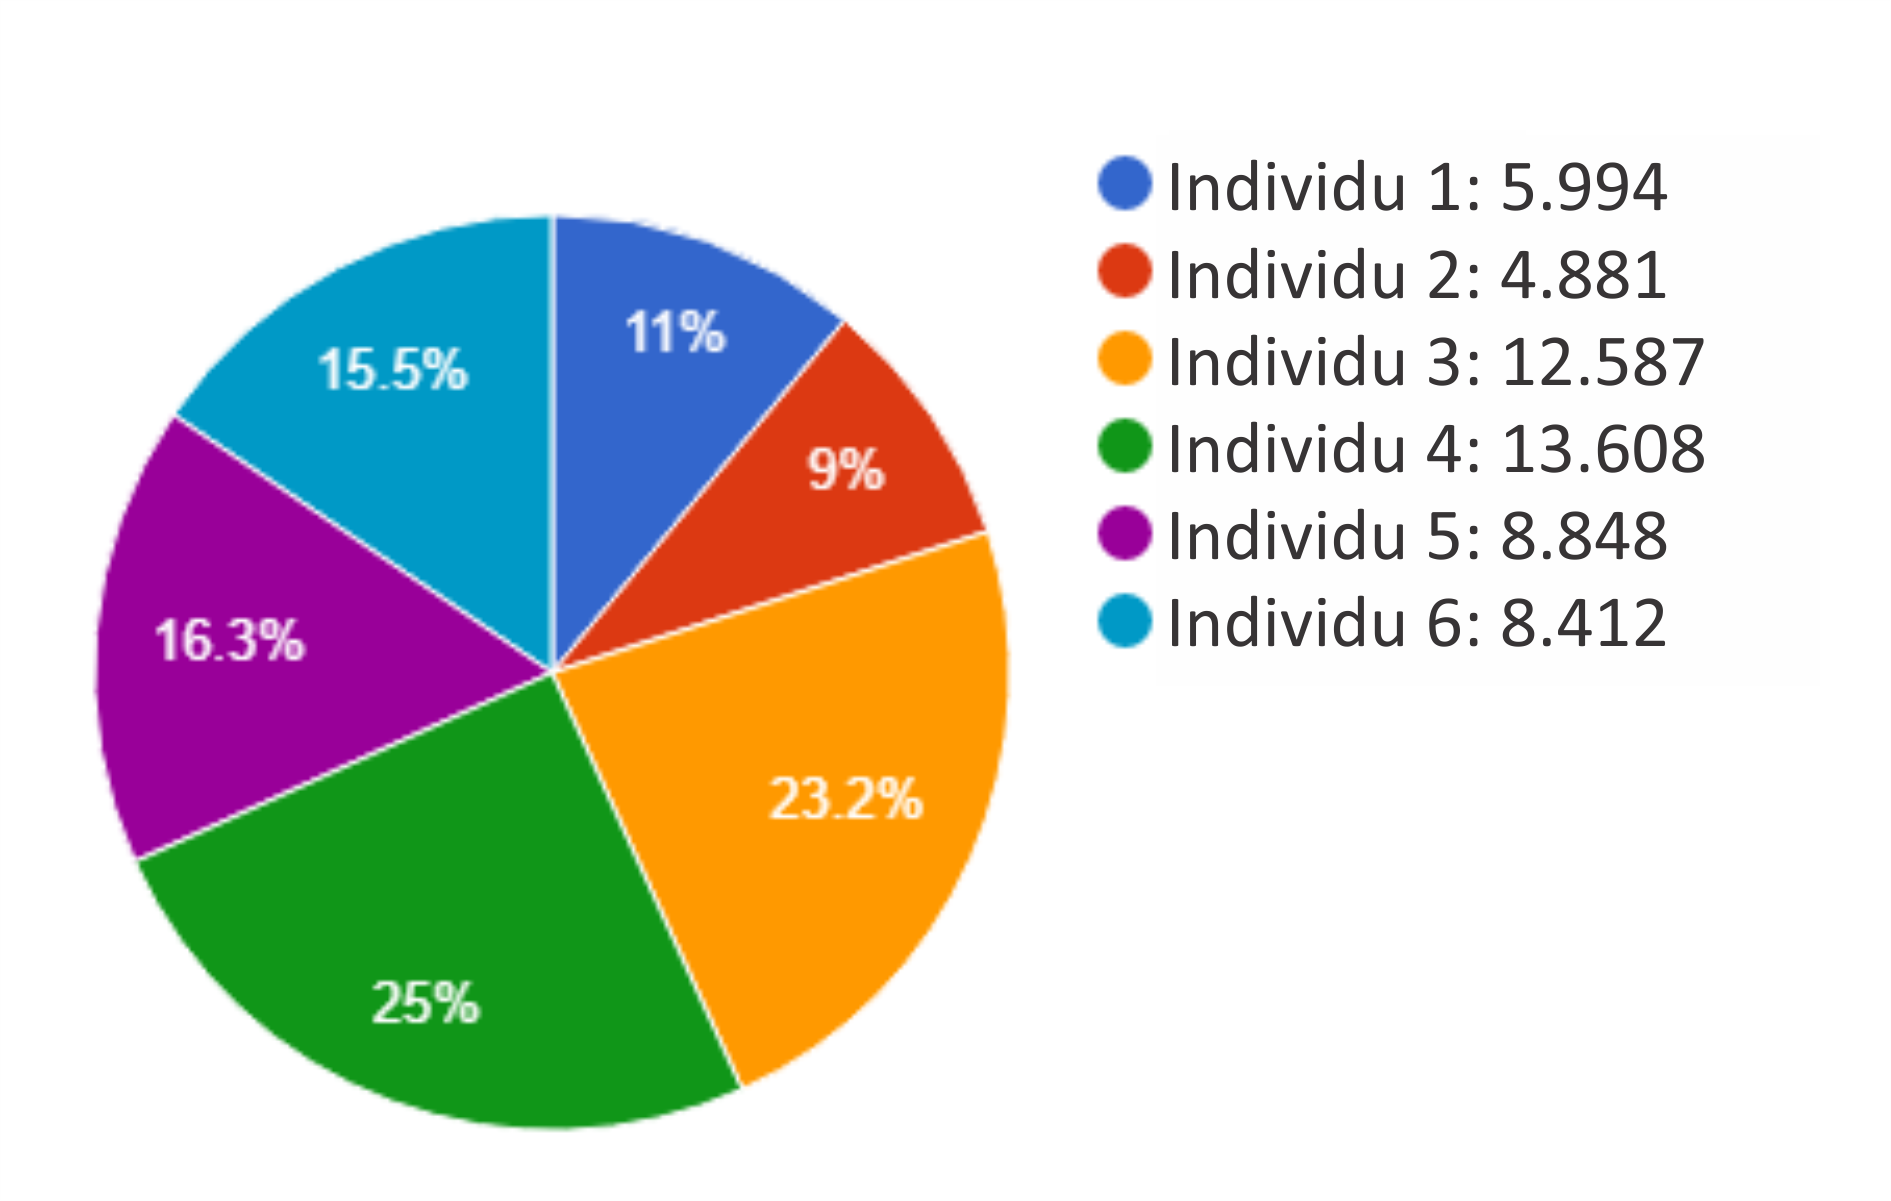
\includegraphics[scale=0.5]{pieChart2}
		\caption{Ilustrasi \textit{roulette-wheel}}
		\label{fig:pieChart}
	\end{center}
\end{figure}

Sebagai penjelasan dari ilustrasi pada Gambar \ref{fig:pieChart} mengenai nilai \textit{fitness} relatif adalah sebagai berikut:
\begin{itemize}
	\item Ada enam individu dalam suatu populasi (Individu 1, Individu 2, dst).
	\item Setiap individu memililiki nilai \textit{fitness} seperti yang tertera pada gambar (Individu 1 memiliki nilai \textit{fitness} sebesar 5.994, Individu 2 memiliki nilai \textit{fitness} sebesar 4.881, dst).
	\item Berdasarkan nilai \textit{fitness} tersebut, maka tiap Individu dalam populasi memiliki peluang terpilih yang tercantum dalam persentase pada diagram lingkaran (Individu 1 memiliki peluang terpilih sebesar 11\%, Individu 2 memiliki peluang terpilih sebesar 9\%, dst). Peluang tersebut dapat dihitung menggunakan persamaan \ref{eq:ProbSelection}.
\end{itemize}

\begin{equation}
	\label{eq:ProbSelection}
	P_i=\frac{f_i}{\sum_{j \in Pop} f_j}
\end{equation}
dengan $P_i$ merupakan peluang terpilihnya individu $i$, $f_i$ merupakan nilai \textit{fitness} dari individu $i$,$Pop$ merupakan populasi, dan $f_j$ merupakan nilai \textit{fitness} dari individu $j$.

Proses seleksi dalam GA akan memilih sejumlah induk yang cukup untuk reproduksi dan membentuk generasi selanjutnya. Untuk meningkatkan performa GA, dapat juga diterapkan strategi \textit{elitism} yaitu dengan langsung memindahkan satu atau beberapa individu dengan nilai \textit{fitness} terbaik ke generasi selanjutnya. Sisanya akan dilakukan dengan cara yang sudah ditentukan sebelumnya seperti \textit{roulette-wheel selection}. Hal ini dilakukan untuk mencegah individu tersebut hilang dari populasi dalam proses reproduksi.

\subsection{Persilangan}
\label{sub:crossover}
Persilangan adalah operasi genetik yang digunakan untuk menggabungkan informasi genetik dari dua induk untuk menghasilkan keturunan baru \cite{sivanandam2007introduction}. Persilangan dilakukan untuk menghasilkan suatu individu baru yang diharapkan memiliki \textit{fitness} yang lebih baik daripada orangtuanya. Salah satu teknik yang dapat digunakan dalam persilangan adalah \textit{Single-point crossover}. Sebuah titik pada kedua induk dipilih untuk menjadi titik persilangan (\textit{crossover point}). Gen yang berada di sebelah kanan titik persilangan bertukar antara kedua kromosom induk seperti yang ditunjukkan pada Gambar \ref{fig:spcrossover}.

\begin{figure}[h]
	\begin{center}
		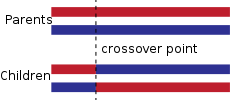
\includegraphics{OnePointCrossover}
		\caption{\textit{Single-point crossover}}
		\label{fig:spcrossover}
	\end{center}
\end{figure}

\subsection{Mutasi}
\label{sub:mutation}
Mutasi adalah suatu operator genetik yang digunakan untuk mempertahankan keragaman genetik dari satu generasi populasi dalam algoritma genetika. Oleh karena itu, mutasi juga dapat mencegah GA terjebak di \textit{local optimum} \cite{sivanandam2007introduction}. Mutasi mengubah satu atau beberapa nilai dalam gen. Mutasi terjadi berdasarkan probabilitas mutasi $\mu_m$ yang sudah ditentukan sebelumnya. Probabilitas mutasi menentukan seberapa sering kromosom akan dimutasi. 

Jika tidak terjadi mutasi, maka keturunannya akan langsung masuk ke populasi setelah persilangan tanpa pengubahan. Apabila terjadi mutasi, satu atau beberapa bagian dari kromosom akan diubah. Mutasi seharusnya tidak dilakukan terlalu sering, karena jika terlalu sering dilakukan maka GA akan menjadi sama dengan algoritma pencarian acak primitif (\textit{primitive random search}). Mutasi akan dilakukan dengan mengubah nilai dari suatu gen yang telah dipilih menjadi nilai lainnya dengan teknik tertentu (tergantung struktur data dari gen yang akan diubah).

\subsection{Proses Pencarian Dalam Algoritma Genetika}
Proses pencarian dalam GA secara umum dijelaskan dalam Algoritma \ref{alg:GA}. Proses pencarian ini memanfaatkan operasi genetik yang telah dijelaskan sebelumnya (Subbab \ref{sub:fitness} sampai dengan Subbab \ref{sub:mutation}). Selain itu, terdapat algoritma lain yang menjelaskan masing-masing operasi genetik yang digunakan dalam Algoritma \ref{alg:GA}. Operasi seleksi yang telah dibahas pada Subbab \ref{sub:selection} dijelaskan pada Algoritma \ref{alg:GA:selection}. Operasi persilangan yang telah dibahas pada Subbab \ref{sub:crossover} dijelaskan pada Algoritma \ref{alg:GA:crossover}. Operasi mutasi yang telah dibahas pada Subbab \ref{sub:mutation} dijelaskan pada Algoritma \ref{alg:GA:mutation}.

\begin{algorithm}[H]
	\caption{Algoritma Genetika \cite{russell2016artificial}}
	\label{alg:GA}
	\begin{flushleft}
		\textbf{function} Algoritma-Genetika(\textit{populasi}) \textbf{returns} solusi berupa individu
		\begin{flushleft}
			\begin{tabular}{ l l }
  				\textbf{input:} & \textit{populasi}, himpunan individu
			\end{tabular}
			\hspace{5pt}  
		\end{flushleft}
	\end{flushleft}
	\begin{algorithmic}[1]
		\STATE $solusi \leftarrow$ \textit{array} yang menyimpan solusi tiap generasi \label{alg:GA:ln-1}
		\REPEAT \label{alg:GA:ln-2}
			\STATE tambahkan individu dengan nilai \textit{fitness} tertinggi dari $populasi$ ke $solusi$ \label{alg:GA:ln-3}
			\STATE $populasi\_baru \leftarrow$ himpunan kosong \label{alg:GA:ln-4}
			\FOR{$i$=1 \textbf{to} Size($populasi$)} \label{alg:GA:ln-5}
				\STATE $x \leftarrow$ Seleksi-acak($populasi$) \label{alg:GA:ln-6}
				\STATE $y \leftarrow$ Seleksi-acak($populasi$) \label{alg:GA:ln-7}
				\STATE $anak \leftarrow$ Persilangan($x$, $y$) \label{alg:GA:ln-8}
				\STATE $rand \leftarrow$ Random(0,1) \label{alg:GA:ln-9}
				\IF{$rand \leq$ $prob\_mutasi$} \label{alg:GA:ln-10}
					\STATE $anak \leftarrow$ Mutasi($anak$) \label{alg:GA:ln-11}
				\ENDIF \label{alg:GA:ln-12}
				\STATE tambahkan $anak$ ke $populasi\_baru$ \label{alg:GA:ln-13}
			\ENDFOR \label{alg:GA:ln-14}
			\STATE $populasi \leftarrow populasi\_baru$ \label{alg:GA:ln-15}
		\UNTIL{$N$ solusi terakhir pada $solusi$ tidak memiliki perubahan yang signifikan} \label{alg:GA:ln-16}
		\STATE \textbf{return} individu terbaik dalam populasi, berdasarkan nilai \textit{fitness} \label{alg:GA:ln-17}
	\end{algorithmic}
\end{algorithm}

Penjelasan untuk fungsi  Algoritma-Genetika pada Algoritma \ref{alg:GA} adalah sebagai berikut:
\begin{itemize}
	\item Pada baris \ref{alg:GA:ln-1}, variabel $solusi$ berfungsi untuk mencatat sejarah dari solusi yang pernah dihasilkan pada setiap generasi.
	\item Pada baris \ref{alg:GA:ln-3}, solusi pada generasi saat ini akan dicatat ke variabel $solusi$.
	\item Pada baris \ref{alg:GA:ln-9}, variabel $rand$ akan berisi bilangan riil antara 0 sampai dengan 1. Bilangan riil ini akan dibangkitkan secara acak dengan distribusi \textit{uniform}.
	\item Pada baris \ref{alg:GA:ln-16}, proses pengulangan akan berhenti saat nilai \textit{fitness} pada $N$ solusi terakhir sudah mengalami konvergensi.
	\item Pada baris \ref{alg:GA:ln-17}, fungsi mengembalikan individu terbaik dalam populasi terakhir GA.
\end{itemize}

\begin{algorithm}[H]
	%fungsi persilangan
	\caption{Persilangan Algoritma Genetika}
	\label{alg:GA:crossover}
	\begin{flushleft}
		\textbf{function} Persilangan($x$,$y$) \textbf{returns} anak berupa individu
		\begin{flushleft}
			\begin{tabular}{ l l }
				\textbf{inputs:}& $x$ dan $y$, individu induk
				\hspace{5pt} 
			\end{tabular} 
		\end{flushleft}
	\end{flushleft}

	\begin{algorithmic}[1]
		\STATE $n \leftarrow$ Length($x$) \label{alg:GA:crossover:ln-1}
		\STATE $c \leftarrow$ Random(1,$N$) \label{alg:GA:crossover:ln-2}
		\STATE \textbf{return} Append(Substring($x$,1,$c$), Substring($y$,$c$+1,$n$)) \label{alg:GA:crossover:ln-3}
	\end{algorithmic}
\end{algorithm}

Penjelasan untuk fungsi Persilangan pada Algoritma \ref{alg:GA:crossover} adalah sebagai berikut:
\begin{itemize}
	\item Pada baris \ref{alg:GA:crossover:ln-2}, variabel $c$ akan berisi bilangan bulat antara 1 sampai $N$. Bilangan bulat ini akan dibangkitkan secara acak dengan distribusi \textit{uniform}.
	\item Pada baris \ref{alg:GA:crossover:ln-3}, \textit{Append} merupakan fungsi untuk menggabungkan dua \textit{string} dan \textit{Substring} merupakan fungsi untuk memotong \textit{string} mulai dari batas tertentu sampai dengan batas tertentu juga.
\end{itemize}

\begin{algorithm}[H]
	%fungsi seleksi acak
	\caption{Seleksi Algoritma Genetika}
	\label{alg:GA:selection}
	\begin{flushleft}
		\textbf{function} Seleksi-acak($populasi$) \textbf{returns} sebuah individu hasil seleksi
		\begin{flushleft}
			\begin{tabular}{ l l }
				\textbf{input:}& $populasi$, populasi saat ini
				\hspace{5pt} 
			\end{tabular} 
		\end{flushleft}
	\end{flushleft}
	
	\begin{algorithmic}[1]
		\STATE $sum \leftarrow$ 0 \label{alg:GA:selection:ln-1}
		\FORALL{$individu \in populasi$ } \label{alg:GA:selection:ln-2}
			\STATE $sum \leftarrow$ $sum$ $+$ Fitness($individu$) \label{alg:GA:selection:ln-3}
		\ENDFOR \label{alg:GA:selection:ln-4}
		\STATE $terpilih \leftarrow$ Random(0,1) $\times$ $sum$ \label{alg:GA:selection:ln-5}
		\FORALL{$individu \in populasi$} \label{alg:GA:selection:ln-6}
			\STATE $terpilih \leftarrow$ $terpilih$ $-$ Fitness($individu$) \label{alg:GA:selection:ln-7}
			\IF{$terpilih \leq 0$ } \label{alg:GA:selection:ln-8}
				\STATE \textbf{return}  $individu$ \label{alg:GA:selection:ln-9}
			\ENDIF \label{alg:GA:selection:ln-10}
		\ENDFOR \label{alg:GA:selection:ln-11}
		\STATE \textbf{return}  individu dengan urutan terakhir di $populasi$ \label{alg:GA:selection:ln-12}
	\end{algorithmic}
\end{algorithm}

Penjelasan untuk fungsi Seleksi-acak pada Algoritma \ref{alg:GA:selection} adalah sebagai berikut:
\begin{itemize}
	\item Pada baris \ref{alg:GA:selection:ln-3}, fungsi \textit{Fitness} akan mengembalikan nilai \textit{fitness} dari individu yang menjadi parameternya.
	\item Pada baris \ref{alg:GA:selection:ln-5}, variabel $terpilih$ akan berisi suatu bilangan 0 sampai $sum$. Hal ini dilakukan dengan cara mengalikan sebuah bilangan riil dengan $sum$. Bilangan riil tersebut merupakan bilangan antara 0 sampai 1 yang dibangkitkan secara acak dengan distribusi \textit{uniform}.
\end{itemize}

\begin{algorithm}[H]	
	%fungsi mutasi
	\caption{Mutasi Algoritma Genetika}
	\label{alg:GA:mutation}
	\begin{flushleft}
		\textbf{function} Mutasi($individu$) \textbf{returns} individu hasil mutasi
		\begin{flushleft}
			\begin{tabular}{ l l }
				\textbf{input:}& $individu$, individu yang akan dilakukan mutasi
				\hspace{5pt} 
			\end{tabular} 
		\end{flushleft}
	\end{flushleft}
	
	\begin{algorithmic}[1]
		\STATE $n \leftarrow$ Length($x$) \label{alg:GA:mutation:ln-1}
		\STATE $c \leftarrow$ Random(1,$n$) \label{alg:GA:mutation:ln-2} 
		\STATE ubah nilai gen ke-$c$ pada $individu$ \COMMENT{nilai bervariasi tergantung metode} \label{alg:GA:mutation:ln-3}
		\STATE \textbf{return} {$individu$} \label{alg:GA:mutation:ln-4}
	\end{algorithmic}
\end{algorithm}

Penjelasan untuk fungsi Mutasi pada Algoritma \ref{alg:GA:mutation} adalah sebagai berikut:
\begin{itemize}
	\item Pada baris \ref{alg:GA:mutation:ln-1}, fungsi \textit{Length} akan mengembalikan panjang dari \textit{string} parameterya.
	\item Pada baris \ref{alg:GA:mutation:ln-2}, fungsi \textit{Random} akan mengembalikan bilangan bulat acak antara 1 sampai $N$.
\end{itemize}

\subsection{GA dalam Pengelompokan}
Algoritma yang umum diterapkan untuk pengelompokan adalah \textit{K-means}. Namun, algoritma \textit{K-means} masih memiliki kekurangan. Salah satu kekurangannya adalah masih dapat terjebak pada \textit{local optimum}. \textit{Local optimum} dapat diatasi oleh GA yang sudah terbukti efektif dalam masalah pencarian dan optimasi \cite{srinivas1994genetic}. Oleh karena itu, diharapkan pengelompokan berbasis GA dapat menghasilkan solusi yang lebih baik dibandingkan dengan algoritma \textit{K-means}.

\section{Model Ruang Vektor}
\label{sec:vsm}
Model ruang vektor adalah representasi dari koleksi dokumen sebagai vektor dalam ruang vektor yang umum \cite{schutze2008introduction}. Model ruang vektor ini biasanya digunakan dalam sejumlah operasi pencarian informasi mulai dari penilaian dokumen pada \textit{query}, klasifikasi dokumen, dan pengelompokan dokumen. Pada penerapannya, akan dilakukan pengukuran kemiripan suatu dokumen terhadap \textit{query} untuk dapat menentukan peringkat relevansi dokumen terhadap \textit{query} (\textit{relevance ranking}). Dokumen dan \textit{query} akan direpresentasikan sebagai model ruang vektor seperti pada Persamaan \ref{eq:vectors}.

\begin{equation}
\label{eq:vectors}
	d_i = (w_{1,i}, w_{2,i}, ..., w_{n,i})
\end{equation}

dengan $d_i$ merupakan dokumen ke-$i$, $w_{n,i}$ merupakan bobot dari \term $n$ untuk dokumen $i$. Setiap dimensi pada vektor tersebut menggambarkan \term berbeda dalam dokumen. Kemiripan antara dokumen dan \textit{query} akan ditentukan dengan mengukur perbedaan sudut antara vektor dokumen dan vektor \textit{query}. Semakin kecil sudut antara dokumen dan \textit{query}, maka dokumen dan \textit{query} dianggap semakin mirip. Namun pada praktiknya, dilakukan perhitungan jarak cosinus untuk menggantikan pengukuran sudut antara dua vektor karena jarak cosinus berbanding terbalik dengan besar sudut antara dua vektor sehingga tidak perlu dilakukan perhitungan lebih lanjut untuk mendapatkan besar sudutnya. Jarak cosinus dapat dihitung menggunakan Persamaan \ref{eq:cosine}.

\begin{equation}
\label{eq:cosine}
s_{ij}=\frac{i\cdot j}{\parallel i \parallel \times \parallel j \parallel}
\end{equation}

dengan $s_{ij}$ adalah kesamaan antara vektor ke-$i$ dengan vektor ke-$j$, $i$ adalah vektor ke-$i$, dan $j$ adalah vektor ke-$j$. Persamaan ini menjelaskan bahwa semakin kecil sudut antara dua vektor, maka tingkat kemiripannya semakin besar.  

\section{Pembobotan \Term (\textit{Term Weighting})}
\label{sec:termWeight}
Suatu dokumen teks terdiri dari deretan karakter. Sebelum suatu dokumen teks dapat diolah informasinya, maka dokumen tersebut perlu melalui suatu proses yang disebut dengan tokenisasi. Menurut \cite{schutze2008introduction}, tokenisasi merupakan proses pemotongan suatu dokumen menjadi potongan-potongan (\textit{token}) tertentu. Pada proses yang sama, karakter tertentu akan turut dibuang (tanda baca, spasi, dll). Token adalah urutan karakter dalam dokumen tertentu yang dikelompokkan bersama sebagai unit semantik. Selain token, terdapat juga istilah yang bernama \textit{type} dan \term. \textit{Type} adalah kelas dari semua token yang berisi urutan karakter yang sama. \Term adalah \textit{type} (mungkin dinormalisasi) yang terdapat pada suatu sistem.

Pembobotan \term merupakan suatu proses menentukan nilai dari suatu \term dalam sebuah dokumen. Pembobotan \term bertugas untuk memetakan \term kepada suatu nilai numerik yang merepresentasikan seberapa penting \term tersebut dalam suatu dokumen. Tidak semua \term dalam dokumen itu penting sehingga dengan memberikan nilai kepada masing-masing \term dapat dengan lebih tepat merepresentasikan isi dokumen. Secara umum, apabila suatu \term semakin penting dalam suatu dokumen (semakin menggambarkan isi dokumen), maka nilai bobotnya akan semakin besar. Sebaliknya jika suatu \term semakin tidak penting (kata-kata yang umum digunakan seperti kata sambung, kata ganti, dan lain-lain), maka nilai bobotnya akan semakin kecil.

Ada beberapa cara untuk menghitung bobot suatu \term. Dua metode yang umum digunakan diantaranya adalah bobot frekuensi (\textit{Frequency weighting}) dan bobot TF-IDF (\textit{TF-IDF weighting}). Bobot TF-IDF merupakan pengembangan dari bobot frekuensi dengan memperhitungkan kemunculan suatu \textit{term} secara global.

\subsection{Bobot frekuensi}
\label{sub:freq}
Bobot frekuensi merupakan teknik pembobotan yang sangat sederhana karena bobotnya merupakan jumlah kemunculan \term tersebut dalam dokumen. \Term yang sering muncul pada suatu dokumen akan dianggap berkaitan dengan dokumen tersebut. Misalkan suatu dokumen banyak memuat \term "properti", maka dokumen tersebut dianggap merupakan suatu dokumen yang membahas masalah "properti". Bobot frekuensi dapat digambarkan dengan Persamaan \ref{eq:bobot}
\begin{equation}
\label{eq:bobot}
w_i=tf_i
\end{equation}
dengan $w_i$ merupakan bobot \term ke-$i$ dan $tf_i$ merupakan frekuensi kemunculan \term ke-$i$ pada dokumen. Sebagai ilustrasi, akan digunakan empat buah dokumen (masing-masing terdiri dari satu kalimat) yang berasal dari contoh pada \cite{schutze2008introduction} sebagai berikut:

%\begin{table}[H]
%	\centering
%	\begin{tabular}{|l|l|c|} \hline
%		& \begin{center} konten \end{center} & panjang dokumen (kata) \\ \hline
%		Doc 1 & new home sales top forecasts & 5 \\ \hline
%		Doc 2 & home sales rise in july & 5\\ \hline
%		Doc 3 & increase in home sales in july & 6 \\ \hline
%		Doc 4 & july new home sales rise & 5\\ \hline
%	\end{tabular}
%\end{table}

\begin{itemize}
	\item Doc 1: new home sales top forecasts
	\item Doc 2: home sales rise in july
	\item Doc 3: increase in home sales in july
	\item Doc 4: july new home sales rise
\end{itemize}

Berdasarkan keempat contoh dokumen, maka dibentuk tabel ketetanggaan antara \textit{term} dengan dokumen pada Tabel \ref{tbl:term-doc}.

\begin{table}[h]
\centering
\begin{tabular}{|l|c|c|c|c|} \hline
	\textit{Term} & d1 & d2 & d3 & d4 \\ \hline
	new		&	1	&	0	&	0	&	1	\\
	home	&	1	&	1	&	1	&	1	\\
	sales	&	1	&	1	&	1	&	1	\\
	top		&	1	&	0	&	0	&	0	\\
	forecast&	1	&	0	&	0	&	0	\\
	rise	&	0	&	1	&	0	&	1	\\
	in		&	0	&	1	&	2	&	0	\\
	july	&	0	&	1	&	1	&	1	\\
	increase&	0	&	0	&	1	&	0	\\ \hline
\end{tabular}
\caption{\textit{Term-document incidence matrix}}
\label{tbl:term-doc}
\end{table}

\Term "\textit{in}" dalam tabel pada d1 dan d4 bernilai 0 karena \term "\textit{in}" tidak muncul pada d1 dan d4. Sedangkan pada d2, \term "\textit{in}" muncul satu kali sehingga bernilai 1 pada tabel. Begitu juga pada d3, \term "\textit{in}" muncul dua kali sehingga bernilai 2 pada tabel.

\subsection{Bobot TF-IDF}
\label{sub:tf-idf}
Selain menggunakan bobot frekuensi, ada teknik pembobotan lain yang disebut dengan TF-IDF (\textit{Term Frequency-Inverse Document Frequency}). Teknik pembobotan ini merupakan pengembangan dari pembobotan frekuensi. TF-IDF merupakang gabungan dari \textit{term frequency} (tf) dengan \textit{inverse document frequency} (idf) untuk menghasilkan suatu bobot komposit untuk setiap \term dalam setiap dokumen \cite{schutze2008introduction}.

\textit{Term frequency} atau biasa dilambangkan sebagai $\textrm{tf}_{t,d}$ untuk \term $t$ pada dokumen $d$. Sama seperti yang telah dijelaskan pada Subbab \ref{sub:freq}, TF merupakan banyaknya kemunculan \term pada suatu dokumen. Namun pada TF-IDF, umumnya digunakan bobot frekuensi yang telah dinormalisasi dengan jumlah kemunculan semua term pada suatu dokumen. TF yang telah dinormalisasi dapat dihitung menggunakan persamaan \ref{eq:tf}.

\begin{equation}
	\label{eq:tf}
	\textrm{tf}_{t,d}=\frac{\textrm{f}_{t,d}}{\sum_{t' \in d}\textrm{f}_{t',d}}
\end{equation}

dengan $\textrm{tf}_{t,d}$ merupakan TF \term $t$ pada dokumen $d$, $\textrm{f}_{t,d}$ merupakan banyaknya kemunculan \term $t$ dalam dokumen $d$, $t' \in d$ merupakan seluruh \term $t'$ yang merupakan anggota dari dokumen $d$, dan $\textrm{f}_{t',d}$ merupakan banyaknya kemunculan \term $t'$ pada dokumen $d$.

Terdapat suatu masalah pada pengukuran menggunakan TF yaitu semua \term dianggap sama penting. Pada kenyatannya, tidak semua \term itu sama penting karena \term yang sangat umum akan memiliki frekuensi yang sangat besar pada banyak dokumen. Seperti yang sudah dijelaskan pada Subbab \ref{sub:freq}, suatu \term yang sering muncul akan dianggap berkaitan dengan suatu dokumen. Namun hal itu ternyata belum tentu benar karena banyak \term yang sering muncul padahal \term tersebut sebenarnya tidak memiliki nilai informasi seperti \term yang merupakan kata penghubung. Oleh karena itu, diperlukan suatu mekanisme untuk mengurangi efek dari suatu \term yang sering muncul di banyak dokumen. Salah satu cara yang digunakan untuk menangani hal tersebut adalah dengan menggunakan \textit{inverse document frequency} (IDF). IDF ini dapat dihitung dengan menggunakan persamaan \ref{eq:idf}.

\begin{equation}
	\label{eq:idf}
	\textrm{idf}_t = \textrm{log} \frac{N}{\textrm{df}_t}
\end{equation}

dengan $\textrm{idf}_t$ merupakan idf dari \term $t$, $N$ merupakan banyaknya anggota himpunan dokumen, dan $\textrm{df}_t$ merupakan \textit{document frequency} dari \term $t$. \textit{Document frequency} adalah banyaknya dokumen pada himpunan dokumen yang memuat \term $t$.

Bobot TF-IDF menggabungkan teknik pembobotan TF dengan IDF. Nilai dari TF digabungkan dengan nilai dari IDF dengan cara mengalikan keduanya. Metode TF-IDF ini sangat populer digunakan oleh sistem rekomendasi berbasis teks \cite{aizawa2003information}. Pembobotan menggunakan TF-IDF dapat dihitung menggunakan Persamaan \ref{eq:tf-idf}.

\begin{equation}
	\label{eq:tf-idf}
	\textrm{tf-idf}_{t,d} = \textrm{tf}_{t,d} \times \textrm{idf}_t
\end{equation}

Berdasarkan rumus tersebut, maka dapat ditarik dua kesimpulan yaitu:
\begin{itemize}
	\item Semakin sering suatu \term muncul di suatu dokumen, maka semakin representatif \term tersebut terhadap isi dokumen.
	\item Semakin banyak dokumen yang memuat suatu \textit{term}, maka nilai informasi \term tersebut semakin kecil. %Hal ini terjadi karena \term yang muncul di mayoritas dokumen tidak dapat menggambarkan arti dari suatu dokumen.
\end{itemize}

Metode penetapan bobot TF-IDF dianggap sebagai metode yang berkinerja baik karena mempertimbangkan frekuensi kemunculan \term baik secara lokal (TF) maupun global (IDF).

\section{Metrik \textit{Intracluster} untuk Mengukur Kinerja Metode \textit{Clustering}}
\label{sec:metric}
Untuk mengukur performa dari suatu algoritma, perlu dilakukan pengujian. Pengujian ini dapat menentukan apakah algoritma yang digunakan sudah cukup baik dalam menyelesaikan masalah yang dibuat. Dalam pengelompokan, ada beberapa cara untuk mengukur apakah objek-objek sudah berhasil dikelompokan secara baik atau tidak. Cara yang pertama adalah dengan mengukur jarak antara tiap objek ke titik pusat \textit{cluster} (\textit{centroid}) atau biasa disebut jarak \textit{intracluster}. Lalu cara yang kedua adalah mengukur jarak antar kelompok yang dapat diukur dengan cara menghitung jarak setiap \textit{centroid} ke \textit{centroid} lainnya.

Metrik yang digunakan \cite{maulik2000genetic} dalam mengukur kinerja suatu metode pengelompokan adalah perhitungan jarak \textit{intracluster}. Jarak \textit{intracluster} dapat diukur dengan cara menjumlahkan jarak setiap objek ke masing-masing titik pusatnya. Cara untuk menghitung jarak \textit{intracluster} ditunjukkan dalam Persamaan \ref{eq:intracluster}.

\begin{equation}
\label{eq:intracluster}
	\begin{gathered}
	M=\sum_{i=1}^K M_i , \\
	M_i=\sum_{x_j\in C_i}\parallel x_j-z_i\parallel
	\end{gathered}
\end{equation}

dengan $M$ merupakan jumlah jarak seluruh objek ke \textit{centroid} masing-masing, $K$ merupakan banyaknya \textit{cluster}, $M_i$ merupakan jumlah jarak seluruh objek anggota \textit{cluster} ke-$i$ ke titik pusatnya, $x_j$ merupakan objek ke-$j$, $C_i$ merupakan \textit{centroid} ke-$i$, dan $z_i$ merupakan \textit{centroid} dari \textit{cluster} ke-$i$. Untuk memperjelas perhitungan, Gambar \ref{fig:intracluster} akan digunakan sebagai ilustrasi dari jarak \textit{intracluster}.

\begin{figure}[h]
	\begin{center}
		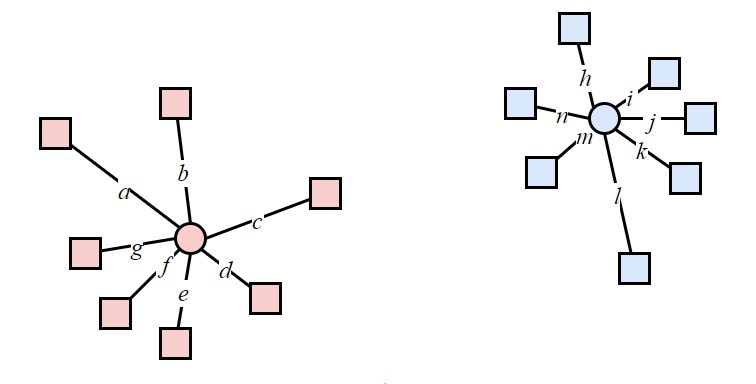
\includegraphics[width=0.6 \textwidth]{intracluster-diagram}
		\caption{\textit{Ilustrasi untuk jarak \textit{intracluster}}}
		\label{fig:intracluster}
	\end{center}
\end{figure}

Pada Gambar \ref{fig:intracluster}, terdapat 14 objek yang telah dibagi ke dalam dua \textit{cluster} berwarna merah dan biru. Persegi pada Gambar \ref{fig:intercluster} mengilustrasikan objek yang akan dikelompokkan. Lingkaran mengilustrasikan titik pusat \textit{cluster} (\textit{centroid}). Garis yang menghubungkan objek dan \textit{centroid} menggambarkan jarak antara objek dengan \textit{centroid} dan ditandai dengan label antara huruf $a$ sampai dengan $n$. Persegi berwarna merah merupakan anggota dari \textit{cluster} 1, sedangkan persegi berwarna biru merupakan anggota dari \textit{cluster} 2. Berdasarkan Persamaan \ref{eq:intracluster}, jarak \textit{intracluster} dari \textit{cluster} 1 ($M_1$) didapat dengan menjumlahkan $a, b, c, d, e, f,$ dan $g$. Sedangkan, jarak \textit{intracluster} dari \textit{cluster} 2 ($M_2$) didapat dengan menjumlahkan $h, i, j, k, l, m,$ dan $n$. Jarak \textit{intracluster} total didapatkan dengan menjumlahkan jarak \textit{intracluster} miliki \textit{cluster} 1 dan \textit{cluster} 2 ($a + b + ... + n$).

Semakin kecil nilai $M$, maka pengelompokan dianggap semakin baik. Ini berarti setiap objek dalam suatu\textit{cluster} mirip satu sama lain. Metrik ini dapat mengukur seberapa baik objek sudah dikelompokan dengan mempertimbangkan kedekatan setiap objek ke titik pusatnya.

\section{Evaluasi Hasil Pengelompokan Menggunakan \textit{Purity}}
Selain metode perhitungan jarak \textit{intracluster} yang telah dijelaskan pada Subbab \ref{sec:metric}, Diperlukan cara eksternal yang dapat mengukur kualitas dari pengelompokan. Pada bagian ini akan dijelaskan salah satu metode eksternal yaitu \textit{purity}. \textit{Purity} adalah persentase objek yang berhasil dikelompokan dengan benar \cite{schutze2008introduction}. Untuk menghitung \textit{purity}, diperlukan suatu \textit{dataset} yang sudah diberi label. Label ini kemudian akan digunakan untuk menghitung akurasi dari pengelompokan itu sendiri. Cara untuk menghitung \textit{purity} ditunjukkan dalam Persamaan \ref{eq:purity}.

\begin{equation}
	\label{eq:purity}
	purity=\frac{1}{N}\sum^k_{i=1} max_j |c_i \cap t_j|
\end{equation}

dengan $N$ merupakan banyaknya objek, $k$ merupakan banyakya \textit{cluster}, $c_i$ merupakan \textit{cluster} ke-$i$, dan $t_j$ adalah label $j$. Rentang dari nilai \textit{purity} adalah antara 0 sampai dengan 1. \textit{Purity} bernilai 1 apabila tidak ada objek dengan 2 atau lebih label berbeda dalam satu kelompok yang sama. Apabila nilai \textit{purity}semakin mendekati 0, maka hasil pengelompokan semakin tidak murni (terdapat banyak objek dengan label berbeda dalam satu kelompok).
